\documentclass{beamer}
\mode<presentation>
\usepackage{amsmath}
\usepackage{amssymb}
\usepackage{adjustbox}
\usepackage{subcaption}
\usepackage{enumitem}
\usepackage{multicol}
\usepackage{mathtools}
\usepackage{listings}
\usepackage{url}
\usepackage{gvv}
\def\UrlBreaks{\do\/\do-}
\usetheme{Boadilla}
\usecolortheme{lily}
\setbeamertemplate{footline}
{
  \leavevmode%
  \hbox{%
  \begin{beamercolorbox}[wd=\paperwidth,ht=2.25ex,dp=1ex,right]{author in head/foot}%
    \insertframenumber{} / \inserttotalframenumber\hspace*{2ex} 
  \end{beamercolorbox}}%
  \vskip0pt%
}
\setbeamertemplate{navigation symbols}{}

\lstset{
frame=single, 
breaklines=true,
columns=fullflexible
}

\numberwithin{equation}{section}

\title{PRESENTATION}
\author{Dwarak A - EE24BTECH11019}
\date{\today} 

\begin{document}

\begin{frame}
\titlepage
\end{frame}

\section*{Outline}
\begin{frame}
\tableofcontents
\end{frame}

\section{Problem Statement}
\begin{frame}
\frametitle{Problem Statement}
Find the maximum and minimum if any for the function
\begin{align}
    f\brak{x} = \sin{\brak{2x}}+5 
\end{align}
\end{frame}

\section{Theoretical Solution}
\subsection{Function and its Derivatives}
\begin{frame}
\frametitle{Function and its Derivatives}
\begin{align}
	f\brak{x} &= \sin{\brak{2x}}+5 \\
	f^\prime\brak{x} &= 2\cos{\brak{2x}} \\
	f^{\prime\prime}\brak{x} &= -4\sin{\brak{2x}}
\end{align}
\end{frame}

\subsection{Critical Points}
\begin{frame}
\frametitle{Critical Points}

To find the critical points, we set the derivative equal to zero:
\begin{align}
	f^\prime\brak{x} &= 0 \\
	\implies 2\cos{\brak{2x}} &= 0 \\
	\implies 2x &= \frac{\pi}{2} + n\pi, \quad n \in \mathbb{Z}\\
	\implies x &= \frac{\pi}{4} + \frac{n}{2}\pi, \quad n \in \mathbb{Z}
\end{align}
\end{frame}

\subsection{Minima, Maxima Condition}
\begin{frame}
\frametitle{Local Minima, Maxima Condition}
Let $A$ be the set of critical points,

For local minima:
\begin{align}
	f^{\prime\prime}\brak{x} &> 0 \\
	\implies -4\sin{\brak{2x}} &> 0 ,\quad x \in A \\
	\implies \sin{\brak{2x}} &< 0 \\
	\implies x_{min} &= \frac{\pi}{4} + \frac{2m-1}{2}\pi, \quad m \in \mathbb{Z} \label{eqn:x_min}
\end{align}
For local maxima:
\begin{align}
	f^{\prime\prime}\brak{x} &< 0 \\
	\implies -4\sin{\brak{2x}} &< 0 ,\quad x \in A \\
	\implies \sin{\brak{2x}} &> 0 \\
	\implies x_{max} &= \frac{\pi}{4} + m\pi, \quad m \in \mathbb{Z} \label{eqn:x_max}
\end{align}
\end{frame}

\subsection{Minimum, Maximum Values}
\begin{frame}
\frametitle{Minimum, Maximum Values}
Minimum value of $f\brak{x}$ using \eqref{eqn:x_min}:
\begin{align}
	f\brak{x_{min}} &= \sin\brak{2x_{min}} + 5 \\
	&= \sin\brak{\frac{\pi}{2} + \brak{2m-1}\pi}, \quad m \in \mathbb{Z} \\
	&= -1 + 5 \\
	&= 4
\end{align}

Maximum value of $f\brak{x}$ using \eqref{eqn:x_max}:
\begin{align}
	f\brak{x_{max}} &= \sin\brak{2x_{max}} + 5 \\
	&= \sin\brak{\frac{\pi}{2} + \brak{2m}\pi}, \quad m \in \mathbb{Z} \\
	&= 1 + 5 \\
	&= 6
\end{align}
\end{frame}

\section{Computational Solution}
\subsection{Gradient Descent and Ascent}
\begin{frame}
\frametitle{Gradient Descent and Ascent}

For the derivative:
\begin{align}
    f^\prime\brak{x_{n}} &= 2\cos{\brak{2x_{n}}}
\end{align}

Gradient Descent to find the local minimum:
\begin{align}
    x_{n+1} &= x_{n} - \eta f^\prime\brak{x_{n}} \\
    x_{n+1} &= x_{n} - 2\eta \cos{\brak{2x_{n}}}
\end{align}

Gradient Ascent to find the local maximum:
\begin{align}
    x_{n+1} &= x_{n} + \eta f^\prime\brak{x_{n}} \\
    x_{n+1} &= x_{n} + 2\eta \cos{\brak{2x_{n}}}
\end{align}

Here, $\eta$ represents the learning rate. The learning rate in gradient descent is a parameter that determines the step size taken in the direction of the negative gradient (for minimization) or the positive gradient (for maximization) during each iteration. $$0 < \eta < 1$$
\end{frame}

\subsection{Parameters and Results}
\begin{frame}
\frametitle{Parameters and Results}

Assuming the following parameters:
\begin{align}
    \eta &= 0.1 \quad\text{(learning rate)} \\
    \text{tolerance} &= 1e-6 \\
    \quad x_{0} &= 0.0 \quad\text{(initial guess)}
\end{align}

The computed results are:
\begin{align}
    x_{\text{min}} &= -0.7853968861361207, \quad y_{\text{min}} = 4.000000000003263 \\
    x_{\text{max}} &= 0.7853968861361207, \quad y_{\text{max}} = 5.999999999996737
\end{align}
\end{frame}


\definecolor{codegreen}{rgb}{0,0.6,0}
\definecolor{codegray}{rgb}{0.5,0.5,0.5}
\definecolor{codepurple}{rgb}{0.58,0,0.82}
\definecolor{backcolour}{rgb}{0.95,0.95,0.95}


\lstset{
    language=C,
    basicstyle=\footnotesize\ttfamily,
    backgroundcolor=\color{backcolour},
    commentstyle=\color{codegreen},
    keywordstyle=\color{blue},
    numberstyle=\tiny\color{codegray},
    stringstyle=\color{codepurple},
    breakatwhitespace=false,
    breaklines=true,
    captionpos=b,
    keepspaces=true,
    numbers=left,
    numbersep=5pt,
    showspaces=false,
    showstringspaces=false,
    showtabs=false,
    tabsize=2
}
\section{C Code}
\begin{frame}[fragile,allowframebreaks]
\frametitle{C Code}
\lstinputlisting[label=mycode1]{codes/gradient.c}
\end{frame}

\definecolor{codegreen}{rgb}{0,0.6,0}
\definecolor{codegray}{rgb}{0.5,0.5,0.5}
\definecolor{codepurple}{rgb}{0.58,0,0.82}
\definecolor{backcolour}{rgb}{0.95,0.95,0.92}

\section{Python Code}
\lstset{
    language=Python,
    basicstyle=\ttfamily\small,
    keywordstyle=\color{blue},
    stringstyle=\color{codepurple},
    commentstyle=\color{codegreen},
    backgroundcolor=\color{backcolour},
    breaklines=true,
    breakatwhitespace=true,
    tabsize=4
}

\begin{frame}[fragile,allowframebreaks]
\frametitle{Python Code}
\lstinputlisting[label=mycode2]{codes/plot.py}
\end{frame}

\section{Plot}
\begin{frame}
\frametitle{Plot}
\begin{figure}[H]
    \centering
	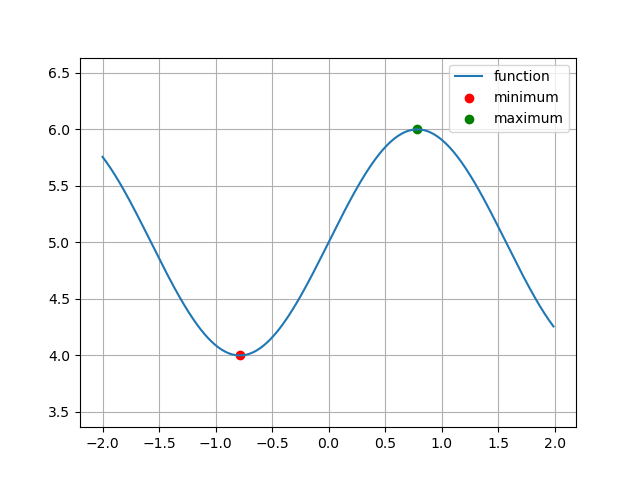
\includegraphics[width=0.7\textwidth]{figs/plot.png}
    \caption{Plot of local maximum and minimum}
    \end{figure}
\end{frame}

\end{document}
